\documentclass[UTF8,10pt]{ctexart}
\usepackage[a4paper,top=13mm,bottom=13mm,left=17mm,right=17mm]{geometry}
\usepackage{amsmath,amssymb,mathtools}
\usepackage{tikz}
\usepackage{enumitem}
\usepackage{microtype}

\pagestyle{empty}
\setlength{\parindent}{2em}
\setlength{\parskip}{0pt}
\linespread{1.08}
\setlist[enumerate]{leftmargin=2.45em,itemsep=1.2pt,topsep=2pt,parsep=0pt}
\newcommand{\blank}{\underline{\hspace{2.8em}}}
\newcommand{\score}[1]{\textbf{（本题满分 #1 分）}}

\begin{document}
\fontsize{12.8pt}{21pt}\selectfont
\begin{center}
  {\fontsize{17.28pt}{21pt}\selectfont\bfseries 2026 年全国中学生数学奥林匹克竞赛（预赛）一试（A卷）\par}
  \vspace{2pt}
  {\kaishu 2026 年 9 月 13 日}\qquad 8:00--9:20
\end{center}
\vspace{2pt}

\noindent\textbf{一、填空题：本大题共 8 小题，每题 8 分，满分 64 分.}
\begin{enumerate}[label=\textbf{\arabic*.},itemsep=5pt]
  \item 平面向量 $\vec x,\vec y,\vec z$ 满足 $|\vec x|=1,|\vec y|=2,|\vec z|=3$，且
  $\vec x\cdot\vec y=\vec x\cdot\vec z=2$，则 $\vec y\cdot\vec z=\blank$.

  \item 设等差数列 $\{a_n\}$ 的公差 $d\ne0$. 若 $a_1,2a_2,4a_4,ta_8$ 成等差数列，则实数 $t=\blank$.

  \item 在 $\triangle ABC$ 中，已知 $\tan A-\cot B=9,\ \tan B-\cot A=13$，则 $\tan C=\blank$.

  \item 对于 $k=0,1,2,\ldots$，定义集合 $A_k=\{20+k,26+2k\}$，并记
  $S_k=A_0\cup A_1\cup\cdots\cup A_k$，则使得集合 $S_n$ 中完全平方数的个数为奇数的最小正整数 $n=\blank$.

  \item 在平面直角坐标系中，双曲线 $\Gamma:\dfrac{x^2}{a^2}-\dfrac{y^2}{b^2}=1\ (a,b>0)$ 经过两点
  $P(1,0),Q(7,12)$，两条（不重合的）平行直线 $l_1,l_2$ 分别经过点 $P,Q$，且 $\Gamma$ 的右焦点 $F$ 到直线
  $l_1$ 的距离等于 $F$ 到直线 $l_2$ 的距离，则 $l_1$ 和 $l_2$ 之间的距离为\blank.

  \item 若复数 $z$ 满足 $\bigl||z|+z\bigr|+z=\mathrm i$，则 $z=\blank$.

  \item 设 $[x]$ 表示不超过实数 $x$ 的最大整数，定义 $\{x\}=x-[x]$. 当 $m,n$ 都是不超过 $30$
  的正整数时，$\left\{\dfrac mn\right\}+\left\{\dfrac nm\right\}$ 的最大值为\blank.

  \item 从一个正方体的 $12$ 条棱中随机选取 $6$ 条，将它们染成红色，则事件“该正方体的 $6$
  个面中，至少有一个面恰含 $2$ 条红色棱”发生的概率是\blank.
\end{enumerate}

\vspace{1pt}
\noindent\textbf{二、解答题：本大题共 3 小题，满分 56 分. 解答应写出文字说明、证明过程或演算步骤.}
\begin{enumerate}[label=\textbf{\arabic*.},start=9,itemsep=10pt]
  \item \score{16} 求最小的实数 $C$，使得存在实数 $x$ 及正实数 $y$，满足
  \[
    \begin{cases}
      2^x+\log_2y=C,\\[-1pt]
      2^{-x}-\log_4y=2C.
    \end{cases}
  \]

  \item \score{20} 在一个底面半径为 $1$、高为 $4$ 的封闭圆柱形容器（容器壁厚度忽略不计）内部有两个半径为 $1$ 的铁球. 设容器内还有若干个大小相同的小钢球与容器的内表面及上述两个铁球都相切. 求小钢球个数的最大可能值.

  \item \score{20} 称满足下述条件 (i) 和 (ii) 的实数列 $a_1,a_2,\ldots,a_m\ (m\geqslant10)$ 是一个 {\kaishu $m$-有趣数列}：

  \hspace{1em}(i) 对任意 $k=1,2,\ldots,m-1$，都有 $|a_{k+1}-a_k|=1$；

  \hspace{1em}(ii) 存在正整数 $i_1,i_2,\ldots,i_{10}\ (i_1<i_2<\cdots<i_{10}\leqslant m)$，使得
  $a_{i_1},a_{i_2},\ldots,a_{i_{10}}$ 成等比数列，且该等比数列的公比 $q\ne\pm1$.

  记 $m_0$ 为使得 $m$-有趣数列存在的最小正整数 $m$. 求 $m_0$ 的值，并确定不同的 $m_0$-有趣数列的个数.
\end{enumerate}

\newpage
\fontsize{12.8pt}{21pt}\selectfont
\begin{center}
  {\fontsize{17.28pt}{21pt}\selectfont\bfseries 2026 年全国中学生数学奥林匹克竞赛（预赛）加试（A卷）\par}
  \vspace{2pt}
  {\kaishu 2026 年 9 月 13 日}\qquad 9:40--12:30
\end{center}
\vspace{5pt}

\noindent\textbf{一、（本题满分 40 分）}\quad
设 $n$ 是正整数，$1=d_1<d_2<\cdots<d_m=n$ 是 $n$ 的所有正约数。已知 $m\geqslant4$，并且对任意
$i,j\in\{1,2,\ldots,m-1\}$，均存在 $k\in\{1,2,\ldots,m\}$，使得 $d_i,d_j,d_k$ 在某种顺序下构成等差数列。求 $m$ 的所有可能值。

\vspace{6pt}
\noindent\textbf{二、（本题满分 40 分）}\quad
如图，在锐角三角形 $ABC$ 中，$AB<AC$，$AD$ 是 $BC$ 边上的高，$H$ 为垂心，$O$ 为外心，$N$ 为 $HO$ 的中点，线段 $BD$ 内一点 $P$ 满足 $\angle PND=2\angle PAD$。

\vspace{0pt}
\noindent\hspace{2em}证明：直线 $BC$ 与三角形 $AOP$ 的外接圆相切。

\begin{center}
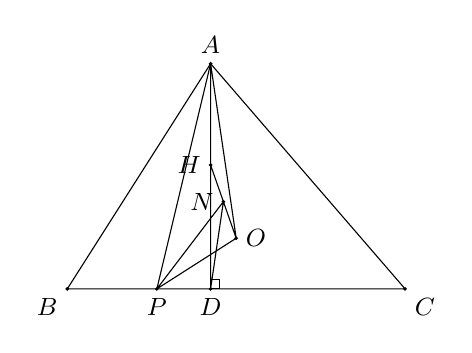
\begin{tikzpicture}[scale=.65,line cap=round,line join=round,every node/.style={font=\small}]
  \coordinate (B) at (0,0);
  \coordinate (C) at (6.6,0);
  \coordinate (D) at (2.8,0);
  \coordinate (A) at (2.8,4.4);
  \coordinate (H) at (2.8,2.42);
  \coordinate (O) at (3.3,.99);
  \coordinate (N) at (3.05,1.705);
  \coordinate (P) at (1.75,0);
  \draw (A)--(B)--(C)--cycle;
  \draw (A)--(D) (A)--(O)--(P)--cycle (H)--(O) (P)--(N)--(D);
  \draw (2.8,0) rectangle +(0.18,0.18);
  \fill (A) circle (1.1pt) (B) circle (1.1pt) (C) circle (1.1pt) (D) circle (1.1pt)
        (H) circle (1.1pt) (O) circle (1.1pt) (N) circle (1.1pt) (P) circle (1.1pt);
  \node[above] at (A) {$A$};
  \node[below left] at (B) {$B$};
  \node[below right] at (C) {$C$};
  \node[below] at (D) {$D$};
  \node[below] at (P) {$P$};
  \node[left] at (H) {$H$};
  \node[left] at (N) {$N$};
  \node[right] at (O) {$O$};
\end{tikzpicture}
\end{center}

\vspace{0pt}
\noindent\textbf{三、（本题满分 50 分）}\quad
设整数 $n>100$，实数 $a_0,a_1,\ldots,a_{n-1}$ 同时满足 (i) 和 (ii)：

\noindent\hspace{2em}(i) $\ 2\geqslant a_0\geqslant a_1\geqslant\cdots\geqslant a_{n-1}\geqslant0$；

\noindent\hspace{2em}(ii) 对任意满足 $0\leqslant i\leqslant j\leqslant k\leqslant n-1$ 且 $i+j+k\geqslant n$ 的整数 $i,j,k$，均有
\[
  a_i a_j+a_j a_k+a_k a_i\leqslant a_i+a_j+a_k.
\]
\noindent\hspace{2em}\begin{tabular}[t]{@{}l@{\quad}l@{}}
  证明： & (1) $a_1+a_2+\cdots+a_{n-1}\leqslant n-1$；\\
         & (2) $a_0+a_1+\cdots+a_{n-1}\leqslant n$。
\end{tabular}

\vspace{4pt}
\noindent\textbf{四、（本题满分 50 分）}\quad
给定整数 $n\geqslant2$。在一个 $4\times n$ 的方格表中，由四个方格构成的下图之一均称为“$S$ 形”。

\begin{center}
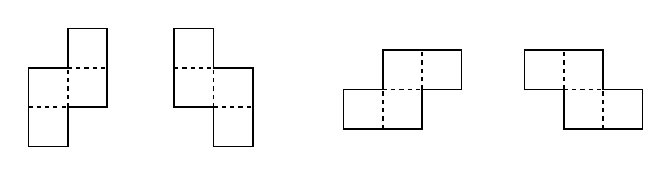
\begin{tikzpicture}[x=5mm,y=5mm,line width=.55pt,dashed/.style={dash pattern=on 1.5pt off 1.5pt}]
  % 竖向 S 形
  \begin{scope}[shift={(0,0)}]
    \draw (0,0)--(1,0)--(1,1)--(2,1)--(2,3)--(1,3)--(1,2)--(0,2)--cycle;
    \draw[dashed] (0,1)--(1,1) (1,1)--(1,2) (1,2)--(2,2);
  \end{scope}
  \begin{scope}[shift={(3.7,0)}]
    \draw (0,1)--(1,1)--(1,0)--(2,0)--(2,2)--(1,2)--(1,3)--(0,3)--cycle;
    \draw[dashed] (0,2)--(1,2) (1,1)--(1,2) (1,1)--(2,1);
  \end{scope}
  % 横向 S 形
  \begin{scope}[shift={(8.0,.45)}]
    \draw (0,0)--(2,0)--(2,1)--(3,1)--(3,2)--(1,2)--(1,1)--(0,1)--cycle;
    \draw[dashed] (1,0)--(1,1) (1,1)--(2,1) (2,1)--(2,2);
  \end{scope}
  \begin{scope}[shift={(12.6,.45)}]
    \draw (0,1)--(1,1)--(1,0)--(3,0)--(3,1)--(2,1)--(2,2)--(0,2)--cycle;
    \draw[dashed] (1,1)--(2,1) (1,1)--(1,2) (2,0)--(2,1);
  \end{scope}
\end{tikzpicture}
\end{center}

\noindent 在方格表中每个方格内填上一个非负实数。已知每个 $S$ 形内四个方格中的数之和均不小于 $1$。求方格表内所有数之和的最小可能值。

\end{document}
